
%%% Local Variables:
%%% mode: latex
%%% TeX-master: "../../doktorarbeit"
%%% End:

\chapter{Supernovae}
The history of supernovae starts, as most astrophysical objects, with observations of strong
electromagnetic events in the night sky. Supernovae are some of the most energetic events
known to astronomers and throughout history some have been clearly visible from earth and could be 
seen even during the day (see \cite{hamacher_14} and references therein). 
The Crab supernova was in 1054 described by Chinese astronomers \citep{ho_96,shen_96}. 
\begin{displayquote}
\textit{... it was visible by day, like Venus; pointed rays shot out
from it on all sides; the color was reddish-white. Altogether it
was visible for 23 days.}
\end{displayquote}
\section{Classifying supernovae}
In the modern era observations of supernovae continually improved. In 1941
German-American astronomer Rudolph Minkowski \citep{minkowski_41} found
that not all supernovae show hydrogen lines in their spectra and
he consequently divided supernovae into two types based on the
presence of hydrogen (Type II) or lack of hydrogen lines (Type I).
Later it was recognized that there were variations within these two classes
and a set of sub-classes, based on variation in the spectra and light curve. 
Type I supernovae were divided into type Ia, Ib and Ic,
where the nebular spectrum of types Ib and Ic was found to be similar to
those of type II supernovae. Two examples of the type II sub-classes are
types II-L and II-P. After reaching the maximum luminosity, the light curves of type II-P supernovae settles onto a
plateau and their luminosity reminds almost constant for several months. The luminosity of Type II-L, on the other hand, 
decline almost linearly. For a detailed reviwe of the classification system see \cite{cappellaro_01}.

The similarities between the nebular spectra of type II and type Ib/c supernovae already hints at a similar 
explosion mechanism. From a theoretical stand point one might say that a classification based on physical processes
powering the supernovae is more prudent. Already in 1960 \cite{hoyle_60} suggested that type II supernovae results from
the implosion of stellar cores and that type I is produced by igniting degenerate stellar material. Today it is understood that
that type Ia supernovae result from the thermonuclear explosions of white dwarfs, in other words the ignition of degenerate stellar material.
Furthermore, we now know that type II and type Ib/c supernovae are the result of the gravitational collapse, the implosion, of stellar cores.
The later category are known as core-collapse supernovae. The subject of this thesis is the gravitational waves generated during the 
collapse and subsequent explosion of a specific sub-type of core-collapse supernova, the ``Iron-core supernova'', and we therefor 
constrain our attention to this class of supernovae. The interested reader is refereed to \cite{janka_12} for a comprehensive description 
of the possible explosion mechanisms.

\section{Iron-core supernovae}
\subsection{Shell burning in massive stars}
\begin{wrapfigure}{r}{0.5\textwidth} \label{figSN:onion}
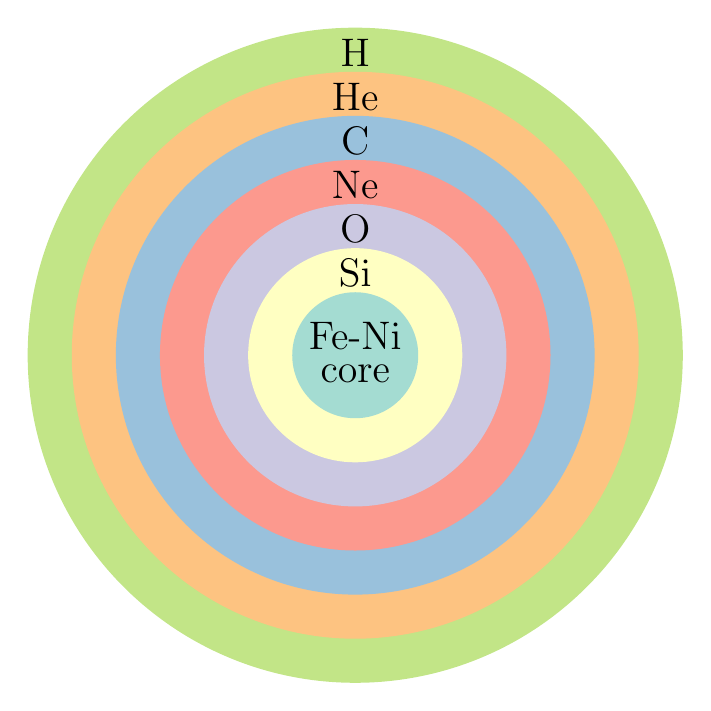
\begin{tikzpicture}[scale=0.8]
\definecolor{c1}{RGB}{141,211,199}
\definecolor{c2}{RGB}{255,255,179}
\definecolor{c3}{RGB}{190,186,218}
\definecolor{c4}{RGB}{251,128,114}
\definecolor{c5}{RGB}{128,177,211}
\definecolor{c6}{RGB}{253,180,98}
\definecolor{c7}{RGB}{179,222,105}
\fill[c7!80] (0,0) circle (5.2cm);
\fill[c6!80] (0,0) circle (4.5cm);
\fill[c5!80] (0,0) circle (3.8cm);
\fill[c4!80] (0,0) circle (3.1cm);
\fill[c3!80] (0,0) circle (2.4cm);
\fill[c2!80] (0,0) circle (1.7cm);
\fill[c1!80] (0,0) circle (1cm);
\node at (0,0.3) {\Large{Fe-Ni}};
\node at (0,-0.3) {\Large{core}};
\node at (0,1.3) {\Large{Si}};
\node at (0,2.) {\Large{O}};
\node at (0,2.7) {\Large{Ne}};
\node at (0,3.4) {\Large{C}};
\node at (0,4.1) {\Large{He}};
\node at (0,4.8) {\Large{H}};
\end{tikzpicture}
\caption{Schematic representation of the shell structure of a massive star right before
the onset of core-collapse. The stellar core consists of consecutive layers where heavier
and heavier elements are burned and a inner iron-nickel core.}
\end{wrapfigure}
When a massive star nears the end of its life it has depleted most of the hydrogen in the central core
and hydrogen burning ceases and the gravitational pull is no longer balanced by radiation pressure resulting
from nuclear fusion. The consequence is that the core starts to contract, the contraction is eventually halted when the pressure
and temperature in the core becomes large enough for helium burning to set in. The layer right outside of the helium burning core is still rich
in hydrogen and so hydrogen burning develops in a layer around the core. The burning of helium in the core stabilises the star, for a while.
However, the helium fuel eventually runs out and the process repeats itself, only this time the contraction continues until carbon ignites in the inner core. 

The process of burning heavier and heavier elements in the core continues up to silicon. The end product of silicon burning is iron-group elements and
since nuclear fusion of iron-group elements does not release any energy the cycle stops at silicon. The end result of this process is
an onion like shell structure consisting of consecutive layers burning heavier and heavier elements. In the centre of this onion is ever growing
core consisting of iron and nickel (hence forth refereed to as the ``iron-core''), it grows due to the ashes produced by the continued burning of silicon in the layer above. A depiction of this shell structure can be seen in \fig{figSN:onion}.
The star remains in this state for a while,
until the central iron-core has accumulated so much matter that its mass exceeds the Chandrasekhar mass and the inevitable gravitational collapse 
of the core begins.
% As John Connor, the star has no hopes of stopping judgement day, it can only hope to postpone it. 
% Gravitational collapse is, as the terminator puts it, inevitable.

\subsection{Iron-core collapse}
The collapse of the iron-core is triggerd and accelarated by two processes.
Firstly, rising temperatures increases the rate of photo-dissociation of iron-group 
nuclei. The nuclei is converted into free nucleons and alpha particles,
witch is a process that consumes thermal energy. Secondly, as the core density increases electron capture
on heavy nuclei becomes more frequent. Free electrons are capture by protons in the nuclei and an neutrons 
and anti-electron neutrinos are produced:
\begin{equation} \label{eqSN:ecapture}
p^{+} + e^{-} \rightarrow n - \bar{\nu}
\end{equation},
were $p^{+}$, $e^{-}$, $n$ and $\bar{\nu}$ represents a proton, an electron, 
a neutron and an anti-electron neutrino, respectively.
The neutrinos escape the core and in the process carry with them energy
and lepton number. With the loss of lepton numbers the mass the pressure from
degenerate electron decreases, effectively reducing the Chandrasekhar mass of the core. 

The deleptonisation of the iron-core eventually stops, at densities around $10^{12}$ g/cm$^3$ the
mean free path of the neutrinos become so short that the time they need to diffuse out of the
core is larger than the time-scale of the collapse. The iron-core, therefor, from this point on collapses in a 
adiabatic and homologous manner. The collapse continues until the central iron-core reaches nuclear densities, around $2.7 \times 10^{14} $g/cm$^3$,
at this point the repulsive forces between nuclei leads to a sudden stiffening of the equation of state (EoS) and the collapse of the
inner iron-core comes to an abrupt halt. 

However, due to its high inertia the inner core contracts beyond the equilibrium point of the
gravitational pull and its new found pressure source. This leads to a recoil and as the inner region of the iron-core expands outwards it crashes
into the infalling material above it. This event is the so called core bounce and it launches a sound wave into the outer iron-core, that 
steepens into a shock wave when it reaches the supersonically infalling layers of the outer core.

As the shock propagates outwards through the dens stellar material it loses about 
$10^{51}$ erg of energy per 0.1 \msun of iron-core material that falls through the shock front, 
due to the dissociation of heavy nuclei, falling through the shock, into free nucleons.
Eventually the density ahead of the shock drops below $\sim \, 10^{11}$ g/cm$^3$ and
the neutrinos behind the shock can suddenly escape. This leads to a burst of neutrino 
emission and a significant loss of energy for the shock. After a few milliseconds the
shock has lost so much energy that it stalls at a radius between 100 and 200 km
and turns into an accretion shock. In order to s



